\section{Installazione ed avvio di SSD}
Per installare ed avviare l'applicativo \gloman{SSD} bisogna effettuare i seguenti passaggi.
\subsection{Scaricare il programma e le librerie}

\begin{itemize}
	\item \textbf{Scaricare}: tutto il programma è presente nel seguente \gloman{Repository}:\newline{}
\centerline{\url{https://github.com/MercurySeven/project-SSD}}

	\item \textbf{Estrarre il contenuto del file .zip}: In una cartella a piacimento, che sia al di fuori della cartella che si vuole sincronizzare, utilizzare l'applicativo del computer per estrarre l'archivio nella cartella desiderata (7zip, WinRAR, etc);
	\item \textbf{Installare le librerie richieste}:
	Tramite terminale, posizionarsi sulla cartella dove è stato estratto il contenuto ed eseguire il seguente comando:\newline{}
	\centerline{\texttt{pip install -r "requirements.txt"}}
\end{itemize}
\subsection{Impostare PYTHONPATH}
Per impostare il PYTHONPATH bisogna utilizzare la keyword set su Windows e la keyword export su macOS e Linux. La variabile deve essere impostata al percorso assoluto dove si è estratto l'archivio.
Di seguito sono riportati due esempi, rispettivamente per Windows e Linux/macOS
\begin{figure}[H]
    \centering
    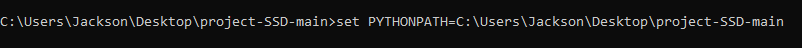
\includegraphics[scale = 0.65]{components/img/Windows-istruzione-1.png}
    \caption{Comando per impostare PYTHONPATH su Windows}
    \label{fig:comando per impostare PYTHONPATH su windows}
\end{figure}
\begin{figure}[H]
    \centering
    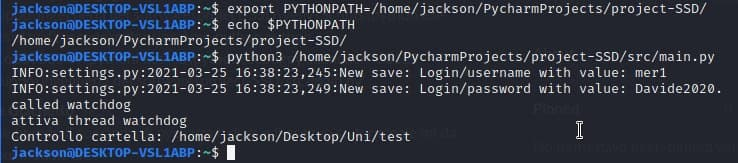
\includegraphics[scale = 0.50]{components/img/linux-istruzione-1.jpg}
    \caption{ Comando per impostare PYTHONPATH su Linux/macOS}
    \label{fig:comando per impostare PYTHONPATH su windows}
\end{figure}
\subsection{Avviare il programma}
Una volta impostato il PYTHONPATH correttamente, per avviare il programma si utilizza il comando python3 seguito dal percorso assoluto del file main.py. Di seguito viene riportato un esempio.
\begin{figure}[H]
    \centering
    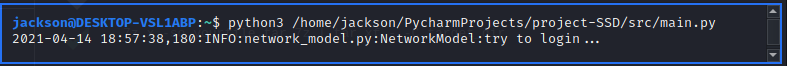
\includegraphics[scale = 0.50]{components/img/avvio.png}
    \caption{Comando per avviare SSD}
    \label{fig:comando per impostare PYTHONPATH su windows}
\end{figure}